\documentclass[11pt]{article}
\usepackage[spanish, es-tabla, es-lcroman]{babel}

%Paquetes básicos
\usepackage{multicol}
\usepackage{physics} 
\usepackage{float}
\usepackage{gensymb}
\usepackage{siunitx} 
\usepackage{enumerate} 
\usepackage{url}
\usepackage{pgfplots}
\usepackage{pgfplotstable}
\usepackage{tikz,pgfplots}
\usepackage{amsmath}  
\usepackage{wasysym} 
\usepackage{geometry}
\usepackage{mdframed}
%Fuente: Helvetica
\usepackage[scaled]{helvet}
\usepackage[T1]{fontenc}
\renewcommand\familydefault{\sfdefault}
\usepackage[eulergreek]{sansmath}
\usepackage[frenchmath]{newtxsf}
\renewcommand{\familydefault}{\sfdefault}
\usepackage{mathastext}
\usepackage{lipsum}
\usepackage{apacite}
\usepackage{natbib}

%Paquetes necesarios para la elaboración de Figuras con el ambiente tikzpicture
\usepackage{tikz} 
\tikzset{font=\fontfamily{phv}\selectfont}
\usepackage{amsmath,tikz}
\usepackage{tikz-3dplot}
\usetikzlibrary{calc,positioning,intersections}
\usetikzlibrary{positioning,shapes.misc}
\tdplotsetmaincoords{80}{120}
\usetikzlibrary{decorations.markings} 
\usetikzlibrary{decorations.pathmorphing}
\usetikzlibrary{shapes, shapes.geometric}
\usetikzlibrary{mindmap,trees}
\usetikzlibrary{backgrounds, fit, positioning}
\tikzstyle{flecha} = [thick,->,>=stealth]


\usepackage{titlesec}
\titleformat{\section}
  {\normalfont\Large\bfseries}{\thesection}{1em}{}


%Geometría de la página y encabezados
\geometry{a4paper,top=3cm,bottom=2.5cm,right=2.5cm,left=2.5cm}
\pgfplotsset{compat=1.14}
\pgfplotsset{/pgf/number format/use comma}
%Estilo de encabezados
\usepackage{fancyhdr}
\pagestyle{fancy}
\fancyhf{}
\lhead{IA Fundamentals}
\rhead{Maestría en CD-IA / UTEC}
\cfoot{\thepage}



%-----------------------
%AQUÍ SE DEBE REEMPLAZAR EL SÍMBOLO NUMERAL POR EL NÚMERO DE LA PRÁCTICA
\chead{Práctica N$^{\circ}$\02}
%-----------------------



%Configuración del estilo de los títulos de las secciones y subsecciones
\usepackage{titlesec}
\titleformat{\section}{\normalfont\normalsize\bfseries}{\thesection.}{0.5em}{}
\titleformat{\subsection}{\normalfont\normalsize\bfseries}{\thesubsection.}{0.5em}{}



%-----------------------
%AQUÍ SE DEBE REEMPLAZAR LO ESCRITO POR EL TÍTULO DE LA PRÁCTICA
\title{\LARGE\textbf{Optimización del Job Shop Problem Usando Hill Climbing y Simulated Annealing}}
%-----------------------



%-----------------------
%Y LOS NOMBRES DE CADA UNO DE LOS INTEGRANTES DEL GRUPO
\author{\normalsize{Silupu Peñaranda, Collin Rodrigo $\cdot$ 202431053}}
%-----------------------


\date{\small{\today}}

\begin{document}
\renewcommand{\BOthers}[1]{et al.\hbox{}}


\maketitle


\hrule
\begin{abstract}
\noindent %En general, el resumen no contiene sangría, el comando noident se encarga de no poner la sangría al párrafo
Este estudio aborda el problema de programación del Job Shop Problem (JSP), un desafío de optimización conocido en el ámbito industrial, que implica la asignación eficiente de recursos compartidos, como máquinas, para completar una serie de trabajos en el menor tiempo de producción posible. La complejidad del JSP radica en su naturaleza combinatoria, que requiere equilibrar múltiples objetivos, como minimizar el makespan y usar eficientemente los recursos. Este documento presenta la aplicación de dos algoritmos de optimización, Hill Climbing y Simulated Annealing, para resolver el JSP. El estudio demuestra que el Simulated Annealing muestra un rendimiento superior al explorar mejor el espacio de soluciones, logrando así un makespan menor. 

\noindent\textit{\textbf{Palabras claves:} Programación de talleres, Hill Climbing, Simulated Annealing.}

\end{abstract}

\hrule

\section{Introducción}

En un mundo cada vez más competitivo, las empresas buscan constantemente maneras de reducir costos y tiempos de producción para mantenerse a la vanguardia. En este sentido, existe una necesidad crítica de ser eficientes en el uso de recursos, lo que lleva al planteamiento del Job Shop Problem (JSP). 

\vspace{1em}
\noindent El JSP es un desafío de optimización conocido por su complejidad en el ámbito industrial. Consiste en la asignación eficiente de recursos compartidos, como máquinas, para completar una serie de trabajos competitivos dentro de un tiempo mínimo de producción. La dificultad del JSP radica en su naturaleza combinatoria, donde la solución óptima debe equilibrar múltiples objetivos, como la minimización del tiempo total de finalización (makespan) y el uso eficiente de recursos energéticos y económicos. Diversas técnicas de optimización, como los algoritmos genéticos, la optimización por colonia de hormigas y la búsqueda tabú, han sido aplicadas para abordar este problema, demostrando mejoras significativas en la productividad y eficiencia industrial \citep{tamssaouet2021, mokhtari2017, musser1993, yusof2011, scalia2023}.

\section{Descripción del JSP}

El JSP consiste en un conjunto \( J = \{J_1, J_2, \ldots, J_n\} \) de \( n \) trabajos y un conjunto \( M = \{M_1, M_2, \ldots, M_m\} \) con \( m \) máquinas. Cada trabajo \( J_i \) tiene \( n_i \) operaciones \( O_{i} = \{O_{i,1}, O_{i,2}, \ldots, O_{i,n_i}\} \). Cada operación \( O_{i,j} \) puede ser realizada por una máquina de un conjunto de máquinas factibles \( M_{i,j} \subseteq M \), para \( 1 \leq i \leq n \) y \( 1 \leq j \leq n_i \). El tiempo de procesamiento de \( O_{i,j} \) en \( M_k \) se representa por \( p_{i,j,k} \) y \( o = \sum n_i \) es el número total de operaciones \citep{escamilla2022}.

\vspace{1em}
\noindent  Es necesario llevar a cabo todas las operaciones para completar un trabajo, respetando la precedencia de operaciones. El JSP tiene las siguientes condiciones: (1) Al inicio, todos los trabajos y todas las máquinas están disponibles. (2) Cada operación solo puede ser realizada por una máquina. (3) Una máquina no puede ser interrumpida mientras procesa una operación. (4) Cada máquina puede realizar una operación a la vez. (5) Una vez definido, el orden de las operaciones no puede ser cambiado. (6) No se consideran fallos de máquinas. (7) Trabajos diferentes no tienen restricciones de precedencia entre ellos. (8) Las máquinas no dependen unas de otras. (9) El tiempo de procesamiento incluye la preparación de las máquinas y la transferencia de operaciones. \citep{escamilla2022}.


\section{Metodología}

Para abordar el JSP, se han desarrollado y aplicado diversos modelos de optimización. En esta sección, se describen dos de estos modelos: Hill Climbing y Simulated Annealing, los cuales han demostrado ser efectivos en la mejora de la productividad y eficiencia industrial.

\subsection{Hill Climbing}
El Hill Climbing es un algoritmo de búsqueda local que itera buscando mejorar una solución actual moviéndose hacia estados vecinos con un valor más alto de una función objetivo. En el contexto del JSP, la función objetivo generalmente es minimizar el tiempo total requerido para completar todas las tareas (makespan). La idea principal detrás de Hill Climbing es siempre moverse hacia una solución vecina que mejore la solución actual. Esto se logra intercambiando tareas o reordenándolas en la secuencia de trabajo para encontrar una configuración que reduzca el makespan \citep{chatgpt}.

\vspace{1em}
\noindent  La función objetivo \( f \) sería: 

    \[
    f: S \rightarrow \mathbb{R}
    \]
    donde \( S \) es el espacio de todas las soluciones posibles y \( f(s) \) mide el makespan de la solución \( s \).

\noindent El vecindario se define con \( N(s) \):
    \[
    N(s) = \{ s' \in S \mid s' \text{ es vecino de } s \}
    \]
donde un vecino \( s' \) se obtiene intercambiando tareas en la secuencia. Asimismo, el algoritmo se puede plantear de la siguiente manera:
    \begin{enumerate}
        \item Inicializar con una solución \( s \).
        \item Mientras no se alcance un criterio de parada:
        \begin{itemize}
            \item Seleccionar \( s' \in N(s) \) tal que \( f(s') < f(s) \) (minimización).
            \item Si no existe tal \( s' \), detenerse.
            \item Si \( f(s') < f(s) \), entonces \( s \leftarrow s' \).
        \end{itemize}
    \end{enumerate}

\subsection{Simulated Annealing}
El Simulated Annealing es un algoritmo de optimización probabilística inspirado en el proceso de enfriamiento de metales. A diferencia de Hill Climbing, este método permite movimientos hacia soluciones peores con una probabilidad decreciente a medida que avanza el tiempo. Esto es particularmente útil en el JSP, ya que el problema a menudo contiene múltiples óptimos locales. El algoritmo explora el espacio de soluciones permitiendo, ocasionalmente, configuraciones que empeoran el makespan actual para escapar de estos óptimos locales y potencialmente encontrar una mejor solución global \citep{chatgpt}.

\vspace{1em} 
\noindent La función objetivo \( f \) sería:
    \[
    f: S \rightarrow \mathbb{R}
    \]
donde \( f(s) \) mide el makespan de la solución \( s \).
El vecindario \( N(s) \) se define como:
    \[
    N(s) = \{ s' \in S \mid s' \text{ es vecino de } s \}
    \]
La temperatura \( T \) se define como:   
    \[
    T: \mathbb{N} \rightarrow \mathbb{R}^+
    \]
La probabilidad de aceptación sería:
    \[
    P(\Delta E, T) = \exp\left(\frac{\Delta E}{T}\right)
    \]
    donde \( \Delta E = f(s') - f(s) \). Asimismo, el algoritmo se puede plantear de la siguiente manera:
    \begin{enumerate}
        \item Inicializar con una solución \( s \) y una temperatura \( T \).
        \item Mientras no se alcance un criterio de parada:
        \begin{itemize}
            \item Generar una solución vecina \( s' \in N(s) \).
            \item Calcular \( \Delta E = f(s') - f(s) \).
            \item Si \( \Delta E \leq 0 \), aceptar \( s' \) como la nueva solución.
            \item Si \( \Delta E > 0 \), aceptar \( s' \) con una probabilidad \( P(\Delta E, T) \).
            \item Reducir la temperatura \( T \).
        \end{itemize}
    \end{enumerate}

\section{Especificación del Problema}
En este apartado se presenta un caso en específico. Se plantea la tarea de organizar y secuenciar 10 trabajos distintos, cada uno compuesto por una serie de operaciones que deben ser realizadas en 4 máquinas diferentes. Cada trabajo debe pasar por todas las máquinas, y cada máquina realiza una operación específica en un tiempo determinado. Las operaciones están detalladas en una matriz donde cada elemento indica en qué máquina se realizará la operación y cuánto tiempo tomará. 

\begin{table}[H]
\centering
\caption{Matriz de trabajos y sus respectivas operaciones en cada máquina}
\[
\begin{array}{c|cccc}
\text{Trabajo} & \text{(Máquina 0, Tiempo)} & \text{(Máquina 1, Tiempo)} & \text{(Máquina 2, Tiempo)} & \text{(Máquina 3, Tiempo)} \\
\hline
0 & (0, 3) & (1, 2) & (2, 2) & (3, 1) \\
1 & (0, 2) & (2, 1) & (1, 4) & (3, 3) \\
2 & (1, 4) & (2, 3) & (0, 2) & (3, 5) \\
3 & (2, 2) & (3, 1) & (0, 4) & (1, 3) \\
4 & (0, 3) & (2, 4) & (3, 2) & (1, 1) \\
5 & (1, 2) & (0, 3) & (3, 4) & (2, 1) \\
6 & (2, 3) & (3, 2) & (0, 1) & (1, 4) \\
7 & (0, 4) & (1, 3) & (2, 2) & (3, 1) \\
8 & (1, 2) & (0, 1) & (3, 4) & (2, 3) \\
9 & (2, 1) & (3, 4) & (0, 3) & (1, 2) \\
\end{array}
\]
\label{tabla:matriz-trabajos}
\end{table}


Por ejemplo, el primer trabajo tiene cuatro operaciones que se realizan en las siguientes máquinas y tiempos:

\begin{multicols}{2}
    
\begin{itemize}
 \item Máquina 0: 3 unidades de tiempo
 \item Máquina 1: 2 unidades de tiempo
 \item Máquina 2: 2 unidades de tiempo
 \item Máquina 3: 1 unidad de tiempo
 \end{itemize}

\end{multicols} 

El objetivo principal de este problema es minimizar el tiempo total necesario para completar todos los trabajos, conocido como makespan. Esto implica encontrar una secuencia óptima en la que los trabajos deben ser procesados en las diferentes máquinas para que el último trabajo se complete en el menor tiempo posible. Para lograr esto, se debe considerar las restricciones de orden de las operaciones dentro de cada trabajo, así como los conflictos que surgen cuando varios trabajos requieren la misma máquina al mismo tiempo. La meta es desarrollar un cronograma eficiente que minimice los tiempos de espera y maximice la utilización de las máquinas, reduciendo así el makespan. Tal y como se mencionó en el apartado anterior, para abordar este problema se aplicarán las técnicas Hill Climbing y Simulated Annealing. 

\section{Resultados}

En este apartado se presentan y analizan los resultados obtenidos al ejecutar los algoritmos de programación implementados para resolver el problema de Job Shop Scheduling. Los métodos empleados incluyen Hill Climbing y Recocido Simulado, cuyas soluciones se evaluarán en términos de makespan y se visualizarán mediante gráficos de Gantt para una mejor interpretación de la asignación de tareas a las máquinas.

\subsection{Hill Climbing}

\begin{figure}[H]
  \centering
  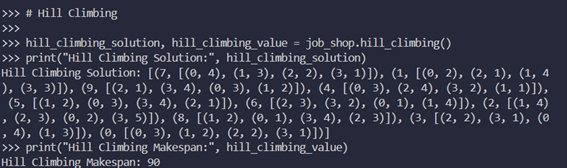
\includegraphics[width=\linewidth]{graphs/Hill Climbing sol.png}
  \label{fig:miImagen}
\end{figure}

\noindent  La solución obtenida utilizando el algoritmo de Hill Climbing presenta una secuencia de trabajos organizada en función del tiempo total requerido por cada uno, comenzando con el trabajo 7 y terminando con el trabajo 0. El makespan obtenido es de 90 unidades de tiempo, lo que indica el tiempo total necesario para completar todos los trabajos en la secuencia determinada.

\vspace{1em} % Esto añade un espacio vertical de 1em entre los párrafos
\noindent  La Figura 1 presenta el gráfico de Gantt. Se observa que cada trabajo está representado por un bloque de color único en el gráfico, mostrando sus operaciones secuenciales en diferentes máquinas. La secuencia de trabajos en el gráfico sigue el orden determinado por el algoritmo de Hill Climbing, empezando con el trabajo 7 y terminando con el trabajo 0. Esto indica que el trabajo 7 tiene la mayor prioridad, seguido por el trabajo 1, y así sucesivamente. En relación a la utilización de cada máquina, se observa que las máquinas están ocupadas durante casi todo el tiempo, con mínimos periodos de inactividad, lo que indica una alta eficiencia en la programación de tareas. Sin embargo, a pesar de la alta utilización de las máquinas, la solución presenta un makespan relativamente alto de 90 unidades de tiempo, lo que sugiere que la secuencia de trabajos podría no ser óptima. Los tiempos de espera entre operaciones dentro de un mismo trabajo pueden estar contribuyendo significativamente a este makespan elevado. Además, el algoritmo Hill Climbing puede quedar atrapado en óptimos locales, limitando su capacidad para encontrar la solución más eficiente. Por lo tanto, aunque la solución muestra una distribución eficiente de las operaciones, existen oportunidades para mejorar el makespan explorando secuencias alternativas o utilizando algoritmos más sofisticados que puedan superar las limitaciones del Hill Climbing.

\begin{figure}[H]
\centering
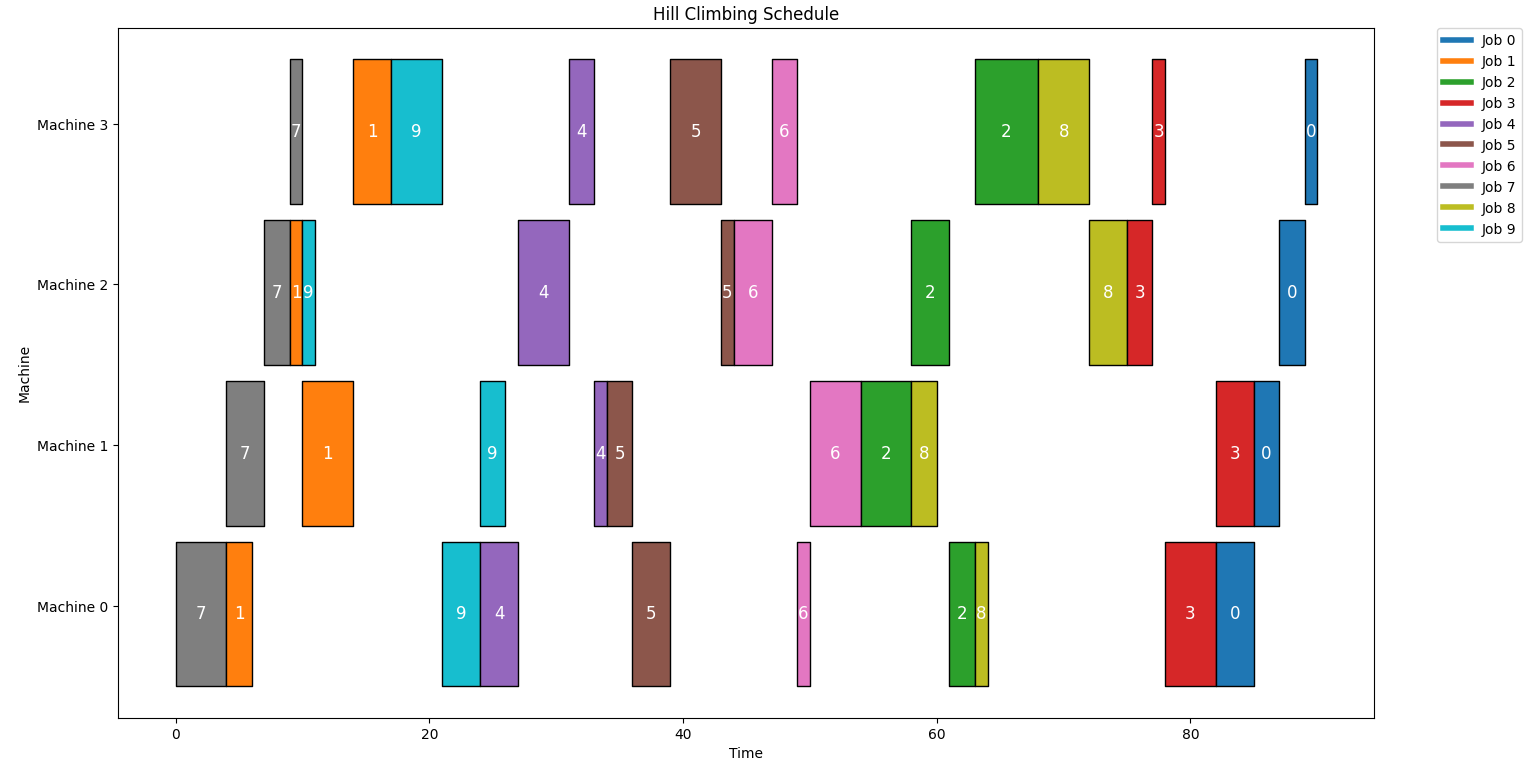
\includegraphics[width=\linewidth]{graphs/Hill Climbing graph.png}
\caption{Gráfico de Gantt para la Solución Obtenida con Hill Climbing}
\label{fig:miImagen}
\end{figure}

\subsection{Simulated Annealing} 

\begin{figure}[H]
  \centering
  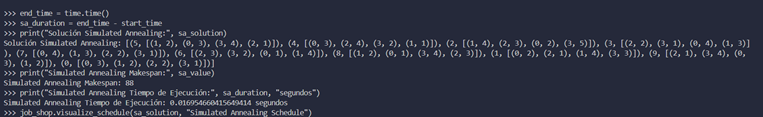
\includegraphics[width=\linewidth]{graphs/Simulated Annealing sol.png}
  \label{fig:miImagen}
\end{figure}

\noindent La solución obtenida utilizando el algoritmo de Simulated Annealing presenta una secuencia de trabajos diferente, organizada de manera que se exploran más combinaciones posibles debido a la naturaleza estocástica del algoritmo. Esta solución comienza con el trabajo 3 y termina con el trabajo 1. El makespan obtenido es de 87 unidades de tiempo, lo que indica una mejora respecto a la solución obtenida con Hill Climbing.

\vspace{1em} % Esto añade un espacio vertical de 1em entre los párrafos
\noindent La Figura 2 presenta el gráfico de Gantt correspondiente. En este gráfico, cada trabajo está representado por un bloque de color único, mostrando sus operaciones secuenciales en diferentes máquinas. La secuencia de trabajos en el gráfico sigue el orden determinado por el algoritmo de Simulated Annealing, comenzando con el trabajo 3 y terminando con el trabajo 1. Esta secuencia permite una mejor distribución de las operaciones, lo que se refleja en el menor makespan. La utilización de cada máquina es alta, con periodos de inactividad mínimos, similar a lo observado con Hill Climbing. Sin embargo, el algoritmo de Simulated Annealing permite aceptar temporalmente soluciones subóptimas para escapar de óptimos locales, lo que resulta en una mejor exploración del espacio de soluciones. Esto se traduce en una distribución más equilibrada de las tareas y una reducción en los tiempos de espera entre operaciones de un mismo trabajo. 

\begin{figure}[H]
\centering
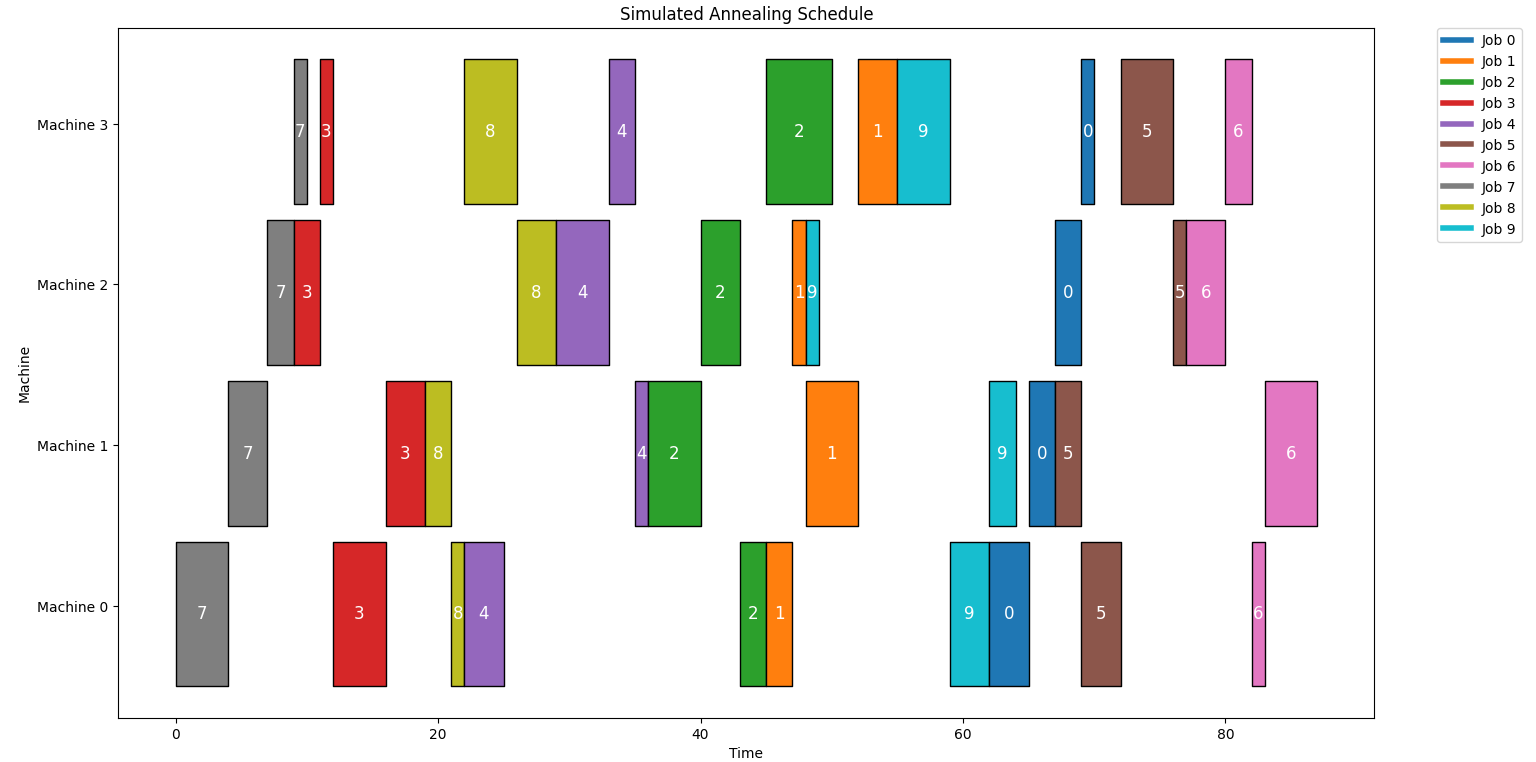
\includegraphics[width=\linewidth]{graphs/Simulated Annealing graph.png}
\caption{Gráfico de Gantt para la Solución Obtenida con Simulated Annealing}
\label{fig:miImagen}
\end{figure}

En este sentido, se observa que, aunque ambas soluciones muestran una alta eficiencia en la utilización de máquinas, la solución de Recocido Simulado es superior al lograr un makespan menor. Este resultado destaca la ventaja del Recocido Simulado en encontrar soluciones más cercanas al óptimo global al equilibrar la exploración y la explotación del espacio de soluciones.

\section{Conclusiones}

En este estudio se abordó el problema de programación de talleres flexibles (JSP) utilizando dos algoritmos de optimización: Hill Climbing y Simulated Annealing. A través de la implementación y análisis de ambos métodos, se obtuvieron soluciones para la secuenciación y asignación de trabajos en múltiples máquinas, con el objetivo de minimizar el tiempo total necesario para completar todos los trabajos, conocido como makespan.

\vspace{1em}
\noindent Los resultados mostraron que:

\begin{itemize}
    \item El algoritmo Hill Climbing, aunque eficiente en la asignación de tareas a las máquinas, tiende a quedar atrapado en óptimos locales, lo que limita su capacidad para encontrar la solución más eficiente. La solución obtenida con este método presentó un makespan de 90 unidades de tiempo.
    \item El algoritmo de Simulated Annealing, por su parte, demostró una mayor capacidad para explorar el espacio de soluciones al aceptar temporalmente soluciones subóptimas. Esto permitió escapar de los óptimos locales y encontrar una mejor secuencia de operaciones, resultando en un makespan de 87 unidades de tiempo, que es inferior al obtenido con Hill Climbing.
\end{itemize}

\noindent Ambos métodos mostraron una alta utilización de las máquinas con periodos mínimos de inactividad, lo que refleja una programación eficiente. Sin embargo, la solución de Simulated Annealing superó a la de Hill Climbing al lograr una mejor distribución de las operaciones y reducir los tiempos de espera entre ellas.

\vspace{1em}
\noindent En conclusión, aunque Hill Climbing es un método sencillo y rápido, el Simulated Annealing demostró ser más eficaz para este tipo de problemas, proporcionando soluciones de mayor calidad al explorar más combinaciones posibles. Para futuros trabajos, se sugiere explorar la combinación de ambos métodos o la aplicación de otros algoritmos de optimización, como los algoritmos genéticos o técnicas de inteligencia artificial, para mejorar aún más los resultados obtenidos y acercarse al óptimo global del problema.



\bibliographystyle{apacite} 
\bibliography{referencias.bib}




\end{document}
